\documentclass[a4paper, 12pt]{article}
\usepackage[T1]{fontenc}
\usepackage{lmodern}
\usepackage{color}
\usepackage{amsfonts}
\usepackage{epstopdf}
\usepackage{matlab}
%\documentclass{book}
\usepackage{blindtext}
\usepackage{hyperref}
\usepackage[brazil]{babel}
\usepackage{amssymb}
\usepackage[utf8]{inputenc}
\usepackage{amsmath}
\usepackage{indentfirst}
\usepackage{graphicx}
\usepackage{multicol,lipsum}
\usepackage[a4paper,
top=3cm, left=3cm, bottom=3cm, right=3cm]{geometry}
\usepackage{setspace}
\usepackage{multirow}
\usepackage{float}
\usepackage[dvipsnames]{xcolor}
\usepackage[table]{xcolor}
%\usepackage{pdflscape}
\usepackage[DIV=15]{typearea}
\usepackage[nottoc]{tocbibind}
\usepackage[sort,numbers]{natbib}
%\usepackage{cite}
\usepackage{matlab}

\usepackage[utf8]{inputenc}
\usepackage[T1]{fontenc}
\usepackage{lmodern}
\usepackage{graphicx}
\usepackage{color}
\usepackage{hyperref}
\usepackage{amsmath}
\usepackage{amsfonts}
\usepackage{epstopdf}
\usepackage[table]{xcolor}
\usepackage{matlab}


\documentclass[letterpaper]{article}
% bib pack %%%%%%%%%%%%%%%%%%%%%%%%%%%%%%%%%%%%%%%%%%%%%%%%%%%%%%%%%%%%%%%%%%%%%
\usepackage[utf8]{inputenc}
\usepackage{geometry}
    \geometry{left=3cm,right=2cm,top=2cm,bottom=2cm}
%
\usepackage[spanish]{babel}
%
\usepackage[fixlanguage]{babelbib}
    \bibliographystyle{babunsrt}
%
\usepackage{url}

\begin{document}
%\maketitle

\begin{titlepage}
	\begin{center}
		

\vspace{10pt}
%\begin{figure}[H][!ht]
%\centering
%
\includegraphics{puc-rio-logo.png}

%\end{figure}
\begin{figure}[!ht]
\centering

\includegraphics{images/puc-rio-logo.png}
\end{figure}
\huge{Fundamentos de Mecatrônica}
        \vspace{70pt}
        
		\textbf{ENG1731}
		\textbf{\large{\\ }}
		
		\vspace{30pt}
		\textbf{\small{\\Lista 03}}
		\vspace{75pt}
		
	\end{center}
	
	\begin{flushleft}
		\begin{tabbing}
		Aluno(a)\qquad\qquad\=\>Paloma Fernanda Loureiro Sette - 1621595\\
			
			Professor(a)\>João Carlos Virgolino Soares\\
	\end{tabbing}
		  
	\end{flushleft}
	\begin{center}
		%\vspace{\fill}
		\vspace{215pt}
		Rio de Janeiro, 26 de Abril de 2023
	\end{center}
\end{titlepage}
%%%%%%%%%%%%%%%%%%%%%%%%%%%%%%%%%%%%%%%%%%%%%%%%%%%%%%%%%%%
\newpage
\tableofcontents
\thispagestyle{empty}

\newpage
\pagenumbering{arabic}

\newpage

%\newcommand{\listequationsname}{Lista de Equações}
%\newlistof{myequations}{equ}{\listequationsname}
%\newcommand{\myequations}[1]{%
%\addcontentsline{equ}{myequations}{\protect\numberline{\theequation}#1}\par}

%\listofmyequations
\newpage


\newpage

\listoffigures
\thispagestyle{empty}

\newpage
%%%%%%%%%%%%%%%%%%%%%%%%%%%%%%%%%%%%%%%%%%%%%%%%%%%%%%%%%
%%%%%%%%%%%%%%%%%%%%%%%%%%%%%%%%%%%%%%%%%%%%%%%%%%%

\newpage

\thispagestyle{empty}

\newpage

\section{Introdução}
Este relatório refere-se ao terceiro trabalho da disciplina de Fundamentos de Mecatrônica, ENG1731, de 2023.1. 

Trataremos da simulação de um sistema mecânico do motor DC brushed Maxon DCX 19 S.

\begin{figure}[H]
\centering
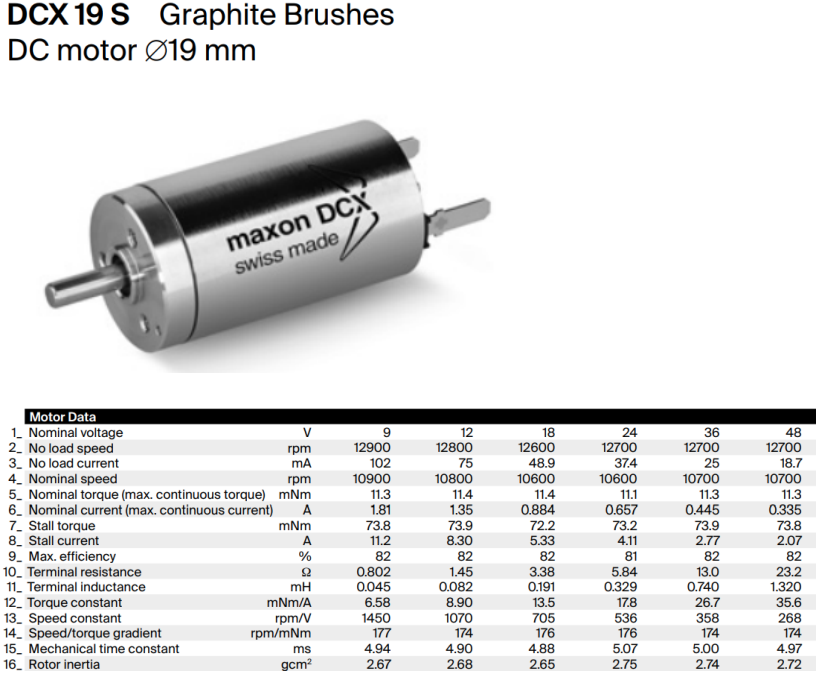
\includegraphics[scale = 0.65]{images/datasheet.png}
\label{filtro1}
\caption{Datasheet do motor DC brushed Maxon DCX 19 S}
\end{figure}

\newpage
\section{Questão 01}
\textbf{Encontre as equações que descrevem a dinâmica do motor usando o modelo de motor de
corrente contínua com campo constante visto na aula 6;} \\

As equações que descrevem a dinâmica do motor DCX 19 S Graphite Brushes usando o modelo de motor de corrente contínua com campo constante são as seguintes:

\subsection{Equação do torque eletromagnético:
}
\begin{equation}
    T_{em} = K_t i   
\end{equation}


Onde:\\

\begin{itemize}
    \item  $T_{em}$ é o torque eletromagnético produzido pelo motor;\\
    \item $K_t$ é a constante de torque do motor, medida em $mNm/A$;
    \item $i$ é a corrente elétrica fornecida ao motor, medida em $A$;\\ 
\end{itemize}

\subsection{Equação da força contra-eletromotriz (back-EMF):}

\begin{equation}
    e_{b} = K_e \omega   
\end{equation}


Onde:\\

\begin{itemize}
    \item $e_{b}$ é a força contra-eletromotriz induzida pelo motor, medida em V;
    \item $K_e$ é a constante elétrica do motor, medida em rpm/V;
    \item $\omega$ é a velocidade angular do motor, medida em $rad/s$.
\end{itemize}



\subsection{Equação do torque de carga:
}

\begin{equation}
    T_{carga} = J \frac{d\omega}{dt} + b \omega
\end{equation}

Onde:\\

\begin{itemize}
    \item $T_{carga}$ é o torque aplicado na carga, medida em mNm;
    \item $J$ é a inércia do rotor do motor, medida em gcm²;
    \item $\frac{d\omega}{dt}$ é a aceleração angular do motor, medida em rad/s²;
    \item $b$ é o coeficiente de atrito viscoso, medida em mNm/(rad/s).
\end{itemize}



\subsection{Modelo Matemático}
\subsubsection{Elétrico}

\begin{equation}
    e_{a} = R_a i_a + e_{b} \>\ \longrightarrow \>\   e_{a} = R_a i_a + K_e \omega
\end{equation}


Onde:\\
\begin{itemize}
    \item $e_{a}$ é a tensão elétrica fornecida ao motor, medida em V;
    \item $R_a$ é a resistência elétrica do motor, medida em $ohm$;
    \item $i_a$ é a corrente elétrica fornecida ao motor, medida em A;
    \item $e_{b}$ é a força contra-eletromotriz induzida pelo motor, medida em V.
\end{itemize}

\subsubsection{Mecânico}

Somatório de torques:

\begin{equation}
    T_{em} =  T_{carga} \>\ \longrightarrow \>\ K_t i_a = J \frac{d\omega}{dt} + b \omega
\end{equation} \\

Sabemos que $\omega = \frac{d\theta}{dt}$, logo, \\

\begin{equation}
    T_{em} =  T_{carga} \>\ \longrightarrow \>\ K_t i_a = J \frac{d \theta^2}{dt} + b \frac{d\theta}{dt}
\end{equation} \\

As equações acima descrevem o comportamento do motor DCX 19 S Graphite Brushes usando o modelo de motor de corrente contínua com campo constante. É importante notar que essas equações são simplificações do comportamento real do motor e podem não levar em conta alguns efeitos não lineares ou não ideais do motor.\\

Portanto, fazendo as substituições necessárias, podemos obter nossa equação geral da dinâmica do motor:

\begin{equation}
    e_{a} = R_a i_a + K_e \frac{d\theta}{dt} \>\ \longrightarrow \>\ i_a = \frac{1}{R_a}e_a - \frac{K_e}{R_a} \frac{d\theta}{dt}
\end{equation}

Substituindo $i_a$ na equação dos torques, teremos:

\begin{equation}
    K_t (\frac{1}{R_a}e_a - \frac{K_e}{R_a} \frac{d\theta}{dt}) = J \frac{d \theta^2}{dt} + b \frac{d\theta}{dt}
\end{equation}

Logo, nossa equação final da dinâmica do motor será:

\begin{equation}
   J \frac{d \theta^2}{dt} =  K_t \frac{1}{R_a}e_a - (K_t \frac{K_e}{R_a} + b) \frac{d\theta}{dt} 
\end{equation} \\

Podemos considerar que:

$\longrightarrow \>\ K_t \frac{K_e}{R_a} + b = B$ \\ 
$\longrightarrow \>\ K_t \frac{1}{R_a} = K$. \\
$e_a$ é nossa entrada e $\frac{d\theta}{dt}$ é nossa saída.

\begin{equation}
   \ddot \theta = \frac{K e_a - B \dot \theta}{J} 
\end{equation} \\


\newpage
\section{Questão 02}
\textbf{Selecione no datasheet os parâmetros necessários para simular o comportamento do motor com uma tensão nominal de 12 V.} \\

Os parâmetros necessários para simular o comportamento do motor com uma tensão nominal de $12V$ são:

\begin{enumerate}
    \item Nominal voltage $(V) = 12$;
    \item No load speed $(rpm) = 12800$;
    \item No load current $(mA) = 75$;
    \item Nominal speed $(rpm) = 10800$;
    \item Nominal torque $(max. continuous torque) (mNm) = 11.4$;
    \item Nominal current $(max. continuous current) (A) = 1.35$;
    \item Stall torque $(mNm) = 73.9$;
    \item Stall current $(A) = 8.30$;
    \item Max. efficiency $(\%) = 82$;
    \item Terminal resistance $(ohm) = 1.45 $;
    \item Terminal inductance $(mH) = 0.082$;
    \item Torque constant $(mNm/A) = 8.90$;
    \item Speed constant $(rpm/V) = 1070$;
    \item Speed/torque gradient $(rpm/mNm) = 174$;
    \item Mechanical time constant $(ms) = 4.90$;
    \item Rotor inertia $(gcm^2) = 2.68$;
\end{enumerate}


\newpage
\section{Questão 03}
\textbf{Simule o comportamento dinâmico do motor escolhido no Simulink utilizando o modelo obtido e os parâmetros do datasheet.
}\\

Teremos a seguinte equação para modelar:

\begin{equation*}
   \ddot \theta = \frac{K e_a - B \dot \theta}{J} 
\end{equation*} \\

\begin{figure}[H]
\centering

\includegraphics[scale = 0.8]{images/simulink.png}
\label{filtro1}
\caption{Modelagem com o Simulink}
\end{figure}


\section{Questão 04}
\textbf{Crie um script no MATLAB para definir os parâmetros do sistema e rodar o Simulink. No script criado, gere gráficos das respostas do sistema. É necessário enviar a resposta do Simulink para o workspace do MATLAB e plotar no script.}


\sloppy
\epstopdfsetup{outdir=./}
\graphicspath{ {./L01_Latex_images/} }

\begin{matlabcode}

%LISTA 03
close all
clear
clc

% Definir os parâmetros do motor
La  = 0.082e-3;         % Indutância (H)
Ra  = 1.45;             % Resistência (Ω)
Kt  = 8.90e-3;          % Constante de torque (Nm/A)
Kv  = 1070*(2*pi)/60;   % Constante de velocidade (rad/s)
Ke  = 1/Kv;

J   = 2.68e-7;
b   = 0.0;

K   = Kt/Ra;
B   = (b+Kt*Ke/Ra);

Ea = 12;                % Tensao nominal (V)

out = sim("simulink_model_L03.slx");

%%
t = out.tout;
w = out.w;

plot(w)
title('Velocidade angular');
xlabel('Tempo (s)');
ylabel("theta'");
grid on;

%%
t1 = out.tout;
w1 = out.w1;

plot(w1)
title('Deslocamento angular');
xlabel('Tempo (s)');
ylabel("theta");
grid on;

%%
t2 = out.tout;
w2 = out.w2;

plot(w2);
title('Corrente');
xlabel('Tempo (s)');
ylabel("ia");
grid on;

%%
t3 = out.tout;
w3 = out.w3;

plot(w3)
title('Torque');
xlabel('Tempo (s)');
ylabel("ia");
grid on;

\end{matlabcode}


Seguem os gráficos gerados através do script do MATLAB, ao enviar a resposta do Simulink para o workspace.

\begin{figure}[H]
\centering
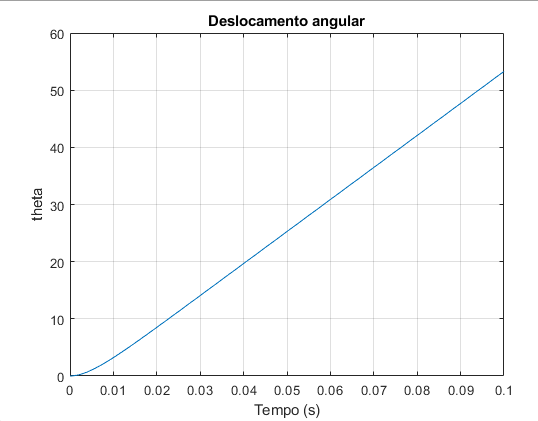
\includegraphics[scale = 0.8]{images/desloc_ang_workspace.png}
\caption{Workspace: gráfico do deslocamento angular em função do tempo}
\end{figure}

\begin{figure}[H]
\centering
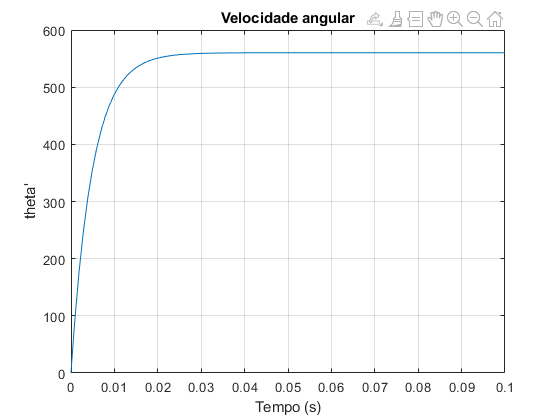
\includegraphics[scale = 0.8]{images/veloc_ang_workspace.png}
\caption{Workspace: gráfico da velocidade angular em função do tempo}
\end{figure}

\begin{figure}[H]
\centering
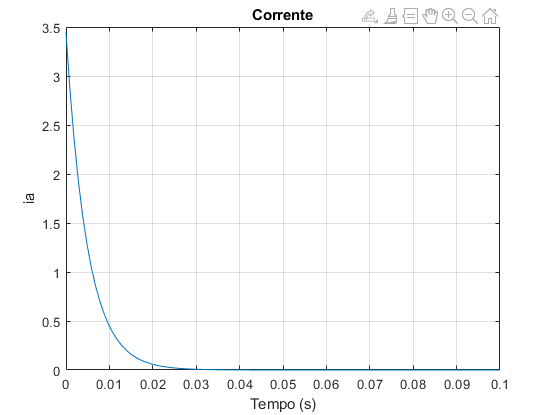
\includegraphics[scale = 0.8]{images/corrente_workspace.png}
\caption{Workspace: gráfico da corrente em função do tempo}
\end{figure}

\begin{figure}[H]
\centering
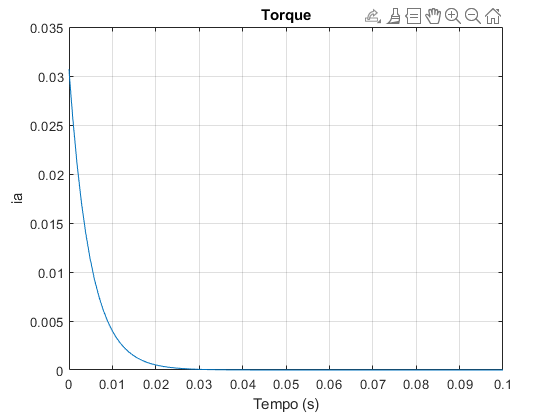
\includegraphics[scale = 0.8]{images/torque_workspace.png}
\caption{Workspace: gráfico do torque em função do tempo}
\end{figure}


\section{Questão 05}
\textbf{Crie as curvas de velocidade angular em função do tempo, torque em função do tempo, corrente em função do tempo. Compare os resultados com os dados do datasheet.}\\

Com o Simulink, geramos as seguintes curvas:

\begin{figure}[H]
\centering
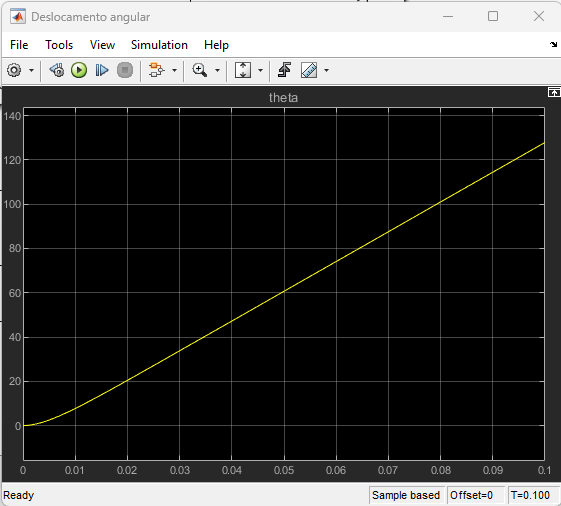
\includegraphics[scale = 0.8]{images/desloc_ang.png}
\label{filtro1}
\caption{Simulink: Deslocamento angular em função do tempo}
\end{figure}

\begin{figure}[H]
\centering
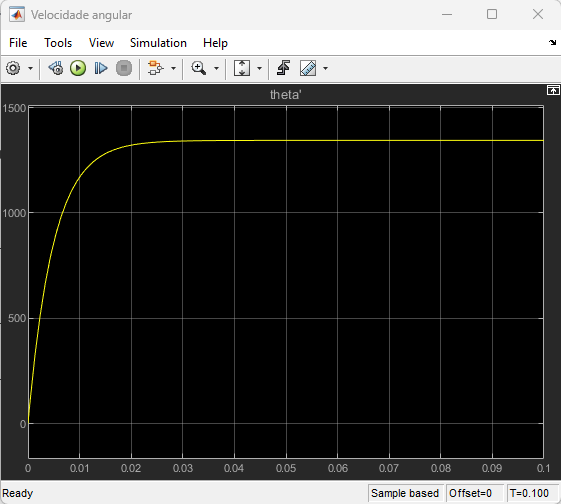
\includegraphics[scale = 0.8]{images/veloc_ang.png}
\label{filtro1}
\caption{Simulink: Velocidade angular em função do tempo}
\end{figure}

\begin{figure}[H]
\centering
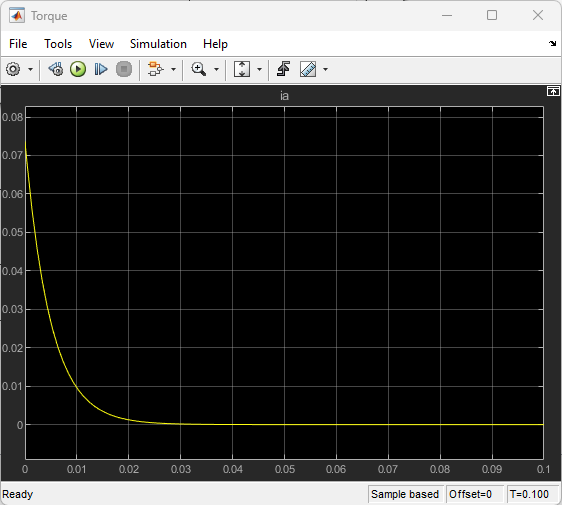
\includegraphics[scale = 0.8]{images/torque.png}
\label{filtro1}
\caption{Simulink: Torque em função do tempo}
\end{figure}


\section{Questão 06}
\textbf{Encontre a resposta analítica (solução particular + homogênea) do modelo matemático, com uma entrada constante de $12V$. Crie no MATLAB a curva de velocidade angular em função do tempo usando a resposta analítica encontrada e compare com a solução numérica do Simulink.}\\


\subsubsection{Solução homogênea:}
Sabemos que \\

\begin{equation*}
    \ddot \theta = \frac{K}{J}e_a - \frac{B}{J} \dot \theta
\end{equation*}

Portanto, nossa solução homogênea será a seguinte:\\

\begin{equation}
    \ddot \theta + \frac{B}{J} \dot \theta = 0
\end{equation} \\

Nossa equação característica será, então: \\

\begin{equation}
    \lambda ^ 2 + \frac{B}{J} \lambda  = 0
\end{equation} \\

Portanto, os polos serão $\lambda_1 = 0 $ e $\lambda_2 = - \frac{B}{J}$. \\

Sabemos que o sistema não é BIBO-estável.  \\

Agora, analisando $\dot \omega$, teremos:

\begin{equation}
    \dot \omega + \frac{B}{J} \omega = 0
\end{equation} \\

Pois, sabemos que $\omega = \dot \theta$. Então, teremos a seguinte equação diferencial:\\ 

\begin{equation*}
    \frac{d \omega}{dt}  = - \frac{B}{J} \omega
\end{equation*}

\begin{equation*}
    \frac{1}{\omega}d\omega  = - \frac{B}{J} dt \>\ \longrightarrow \>\ \int \frac{1}{\omega}d\omega = \int -\frac{B}{J}dt
\end{equation*}

\begin{equation*}
    \ln{\omega} = - \frac{Bt}{J} + C \>\ \longrightarrow \>\ \omega = C e^{-\frac{Bt}{J}}
\end{equation*}

\subsubsection{Solução particular:}

Para encontrar a solução particular, sabemos que temos uma entrada constante de $12V$, que representa a tensão aplicada no motor. Portanto, podemos considerar que a solução particular é uma função linear que depende da entrada: 

\begin{equation}
    \omega_p = k e_a
\end{equation}

Substituindo na equação diferencial, temos:

\begin{equation}
    \ddot{\theta} = \frac{K}{J} e_a - \frac{B}{J} \dot{\theta} = \frac{K}{J} e_a - \frac{B}{J}(\dot{\omega_p}+\dot{\omega_h}) = \frac{K}{J} e_a - \frac{B}{J}(\frac{d}{dt}(ke_a)+\dot{\omega_h}) = \frac{K}{J} e_a - \frac{Bk}{J}(\frac{d}{dt}e_a+\dot{\omega_h}) 
\end{equation}

Assim, precisamos encontrar um valor de $k$ que anule a parte homogênea da solução, ou seja, que satisfaça a equação $\dot{\omega_h} + \frac{B}{J}\omega_h = 0$. Temos que $\omega_h = C e^{-\frac{Bt}{J}}$, portanto, 

\begin{equation}
    \dot{\omega_h} + \frac{B}{J}\omega_h = -\frac{BC}{J}e^{-\frac{Bt}{J}} + \frac{BC}{J}e^{-\frac{Bt}{J}} = 0
\end{equation}

Assim, $C=B/J$. Substituindo na equação da solução particular, temos:

\begin{equation}
    \ddot{\theta} = \frac{K}{J} e_a - \frac{B^2}{JK} e_a = (\frac{K}{J} - \frac{B^2}{JK}) e_a \Rightarrow k = \frac{J}{K-B^2/J}
\end{equation}

Então, a solução geral do sistema com entrada constante é: 

\begin{equation}
    \omega(t) = \omega_h(t) + \omega_p(t) = C e^{-\frac{Bt}{J}} + \frac{J}{K-B^2/J} e_a
\end{equation}

\subsubsection{Solução numérica no Simulink:}

A solução numérica no Simulink pode ser obtida usando o modelo matemático do sistema e uma entrada constante de $12V$. Para isso, podemos definir a entrada como uma constante controlada com um bloco "Constant". O modelo do sistema é dado pelo arquivo "simulink_model_L03.slx". Ao simulá-lo com a entrada constante de $12V$, obtemos uma curva da velocidade angular em função do tempo.

\subsubsection{Resposta analítica no MATLAB:}
Podemos criar a curva da velocidade angular em função do tempo usando a resposta analítica encontrada. Para isso, podemos usar o código abaixo no MATLAB:


\sloppy
\epstopdfsetup{outdir=./}
\graphicspath{ {./L01_Latex_images/} }

\begin{matlabcode}

close all
clear
clc

% Definir os parâmetros do motor
La  = 0.082e-3;         % Indutância (H)
Ra  = 1.45;             % Resistência (Ω)
Kt  = 8.90e-3;          % Constante de torque (Nm/A)
Kv  = 1070*(2*pi)/60;   % Constante de velocidade (rad/s)
Ke  = 1/Kv;

J   = 2.68e-7;
b   = 0.0;

K   = Kt/Ra;
B   = (b+Kt*Ke/Ra);

Ea = 12;                % Tensao nominal (V)

% Encontrar a velocidade angular em função do tempo (resposta analítica)
t = linspace(0, 1, 1000); % tempo em segundos
C = B/J;
k = J/(K-B^2/J);
w_h = C*exp(-B*t/J);
w_p = k*Ea;
w_a = w_h + w_p;

% Simular a curva da velocidade angular em função do tempo (resposta numérica)
out = sim("simulink_model_L03.slx");
t_s = out.tout;
w_s = out.w;


%% Plotando as curvas de velocidade angular em função do tempo
plot(w_a)
xlabel('Tempo (s)')
ylabel('Velocidade angular (rad/s)')
title('Resposta analítica')
grid on

plot( w_s)
xlabel('Tempo (s)')
ylabel('Velocidade angular (rad/s)')
title('Resposta numérica')
grid on

\end{matlabcode}



Este código define os parâmetros do sistema e usa a resposta analítica para obter a curva da velocidade angular em função do tempo. Em seguida, o modelo matemático do sistema é simulado no Simulink para obter a resposta numérica. As duas curvas são plotadas para comparação. \\

As soluções forem coerentes, pois as curvas são semelhantes. Abaixo, podemos ver o resultado da geração da curva de velocidade angular gerado com a resposta analítica pelo MATLAB.\\


\begin{figure}[H]
\centering
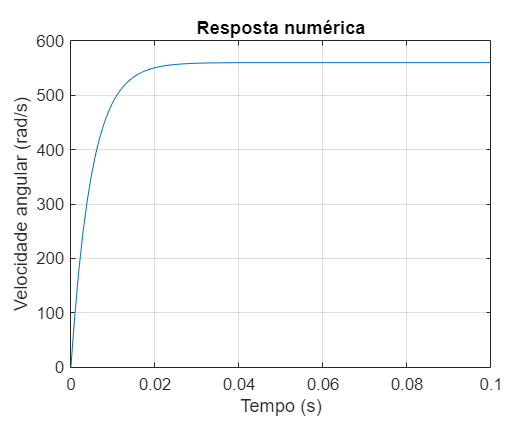
\includegraphics[scale = 0.8]{images/resp_num_script02.png}
\label{filtro1}
\caption{Gráfico gerado da velocidade angular com a resposta analítica no MATLAB}
\end{figure}

\newpage
% REFERENCIAS %%%%%%%%%%%%%%%%%%%%%%%%%%%%%%%%%%%%%%%%%%%%%%%%%%%%%%%%%%%%%%
    \nocite{*}
    \bibliography{src/bibliography}
    
\end{document}
\section{Referências Bibliográficas}



\end{document}